\chapter{Materiales inorgánicos y nanomateriales}\label{ch:b3:inorganic-materials}

Una placa de \omterm{def:b3:inorganic-materials:sol-gel}{aerogel} de sílice, un sólido que es casi todo aire, sostiene una flor sobre la llama
de un gas sin dejar que se marchite. Es un vidrio, obtenido no fundiendo arena sino
dejando que un líquido cuaje en un \omterm{def:b3:colloids:colloid}{gel} y secando después el \omterm{def:b3:colloids:colloid}{gel} sin dejar que
se desplome. La química de materiales trabaja en ese orden: elegir la estructura, después
la vía que la produce, y leer luego las propiedades. Este capítulo recorre
las vías hacia los sólidos inorgánicos, las estructuras de las \omterm{def:b3:inorganic-materials:ceramic}{cerámicas}, los vidrios y los cristales
porosos, y lo que le ocurre a la materia cuando una partícula mide solo unos pocos nanómetros.

\begin{recall}
El volumen del primer año describió los tipos de estructura cristalina, los sitios intersticiales,
los alótropos, el grafito y el diamante; el volumen del segundo año, los diagramas de fases, la temperatura
de transición vítrea y los polímeros. El \cref{ch:b3:surfaces-catalysis} definió la
\omterm{def:b3:surfaces-catalysis:surface-area}{superficie específica}; el \cref{ch:b3:colloids}, los \omterm{def:b3:colloids:colloid}{soles} y los \omterm{def:b3:colloids:colloid}{geles};
el \cref{ch:b3:solid-state}, las bandas, los \omterm{def:b3:solid-state:defects}{defectos puntuales} y los \omterm{def:b3:solid-state:ionic-conductor}{conductores iónicos};
el \cref{ch:b3:quantum-model-systems} resolvió la \omterm{def:b3:quantum-model-systems:box}{partícula en una caja}, y
el \cref{ch:b3:point-groups} dio el grupo icosaédrico.
\end{recall}

\begin{omfigure}
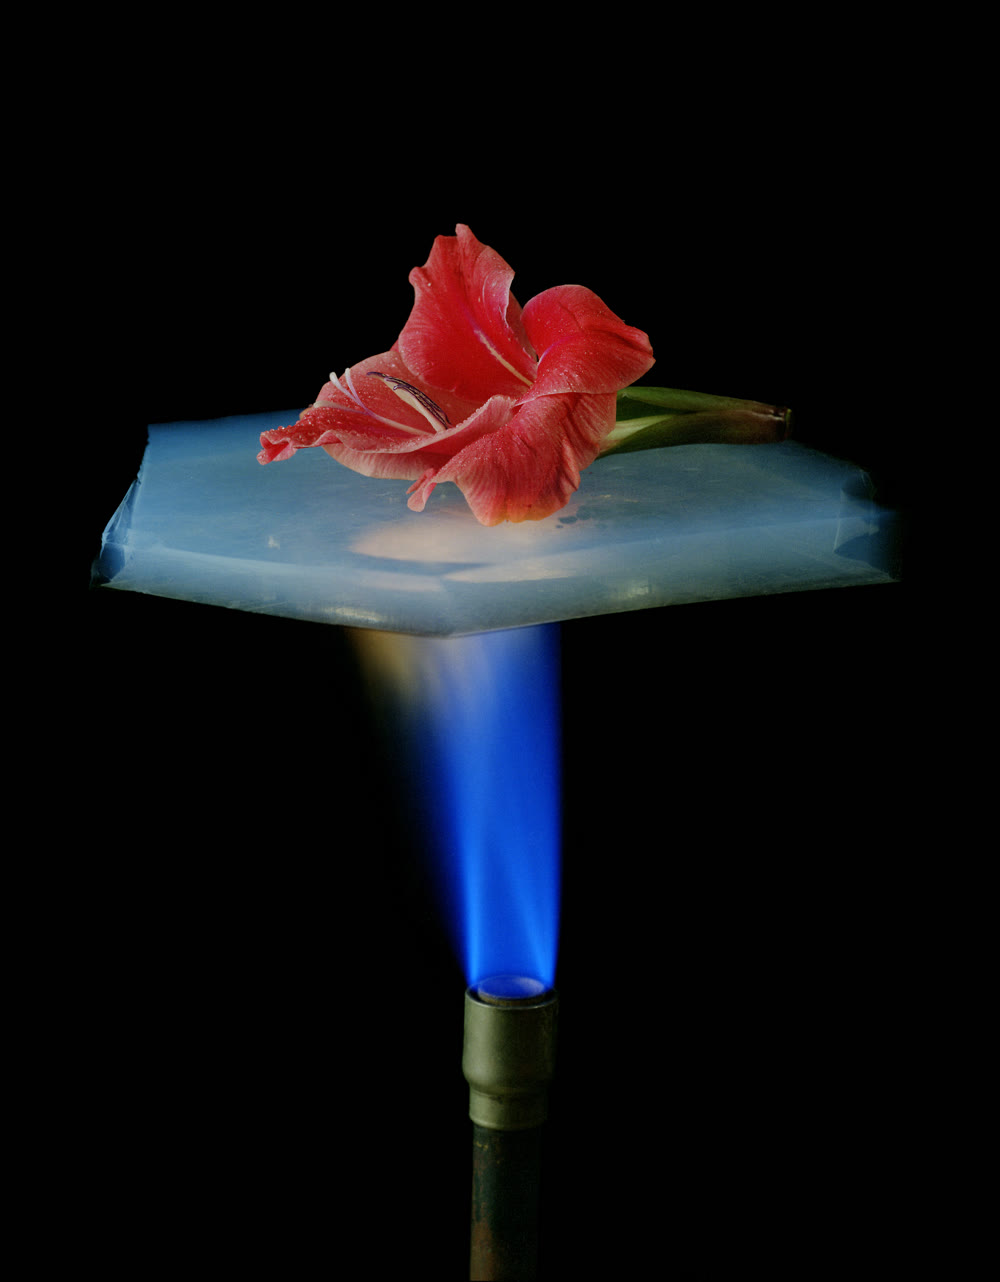
\includegraphics[width=0.38\linewidth]{images/book4/aerogel-flower.jpg}

{\small Una flor sobre una placa de \omterm{def:b3:inorganic-materials:sol-gel}{aerogel} de sílice encima de la llama de un gas: el \omterm{def:b3:inorganic-materials:sol-gel}{aerogel}, un
\omterm{def:b3:colloids:colloid}{gel} seco que es casi todo espacio vacío, conduce muy mal el calor. Fotografía:
NASA/JPL, dominio público.}
\end{omfigure}

\section{Vías de síntesis}

\begin{definition}[Método cerámico]\label{def:b3:inorganic-materials:ceramic-method}
El \emph{método cerámico}\index{metodo ceramico@método cerámico} prepara un compuesto sólido
moliendo juntos los reactivos sólidos y calentándolos, a menudo durante días y
con moliendas intermedias, a temperaturas lo bastante altas para que los iones difundan a través de los
sólidos.
\end{definition}

La reacción entre dos sólidos ocurre en su contacto, y el producto forma una
capa entre ellos que los iones deben atravesar después: la etapa más lenta
es la difusión, que se ralentiza a medida que la capa se engruesa.

\begin{proposition}[Crecimiento parabólico]\label{prop:b3:inorganic-materials:parabolic}
Si el crecimiento de una capa de producto está limitado por la difusión a través de ella, su
espesor crece como $x^2 = kt$.
\end{proposition}

\begin{proof}
Con concentraciones fijas en las dos caras de la capa, el flujo a través de ella
sigue la ley de Fick, $J = D\Delta c/x$. La capa crece en proporción al flujo:
$\dd x/\dd t = \lambda J = \lambda D\Delta c/x$, donde $\lambda$ es el volumen de producto por mol transportado. Entonces
$x\,\dd x = \lambda D\Delta c\,\dd t$, e integrando desde $x = 0$ en $t = 0$ se obtiene $x^2 = 2\lambda D\Delta c\,t = kt$.
\end{proof}

Duplicar el tamaño de las partículas multiplica así por cuatro el tiempo de reacción: de ahí
la molienda fina, la mezcla a escala atómica en un precursor (un oxalato mixto o un \omterm{def:b3:colloids:colloid}{gel}
de citrato que se descompone en el producto deseado) o una vía en disolución.

\begin{definition}[Proceso sol--gel]\label{def:b3:inorganic-materials:sol-gel}
El \emph{proceso sol--gel}\index{proceso sol--gel} prepara un óxido por
hidrólisis y condensación de precursores moleculares, normalmente alcóxidos, en
disolución: la disolución se convierte en un \omterm{def:b3:colloids:colloid}{sol} de pequeños agregados de óxido y después en un \omterm{def:b3:colloids:colloid}{gel}, una
red sólida continua llena de líquido. Secado por evaporación, el \omterm{def:b3:colloids:colloid}{gel}
se contrae en un \emph{xerogel}\index{xerogel} denso; secado por encima del punto
crítico del líquido, lo que lo elimina sin interfase líquido--gas, conserva
su volumen en forma de \emph{aerogel}\index{aerogel}.
\end{definition}

\begin{omfigure}
\setchemfig{atom sep=2.0em}
\schemestart
\chemfig{RO-Si(-[2]OR)(-[6]OR)-OR}
\+ \chemfig{H_2O}
\arrow{->[hidrólisis]}[,1.4]
\chemfig{RO-Si(-[2]OR)(-[6]OR)-OH}
\+ ROH
\schemestop
\par\bigskip
\schemestart
\chemfig{{\equiv}Si-OH}
\+
\chemfig{HO-Si{\equiv}}
\arrow{->[condensación]}[,1.6]
\chemfig{{\equiv}Si-O-Si{\equiv}}
\+ \chemfig{H_2O}
\schemestop
\par\medskip

{\small Química sol--gel de un alcóxido de silicio (R: un grupo alquilo, etilo en el
ortosilicato de tetraetilo): el agua sustituye los grupos alcoxi por grupos hidroxi, y
dos silanoles se condensan en un puente siloxano. Repetidas, las condensaciones construyen
una red tridimensional de sílice.}
\end{omfigure}

Las dos reacciones juntas dan, para una reacción completa,
$\ce{Si(OC2H5)4 + 2H2O -> SiO2 + 4C2H5OH}$. La catálisis ácida hace rápida la hidrólisis y lenta la
condensación, lo que da polímeros finos de tipo cadena; la catálisis básica, lo
contrario, lo que da partículas densas. Los recubrimientos (capas antirreflejo sobre vidrio)
se obtienen sumergiendo una pieza en el \omterm{def:b3:colloids:colloid}{sol} y extrayéndola.

\begin{definition}[Síntesis hidrotermal]\label{def:b3:inorganic-materials:hydrothermal}
La \emph{síntesis hidrotermal}\index{sintesis hidrotermal@síntesis hidrotermal} cristaliza un
sólido a partir de agua por encima de su punto de ebullición normal, en un recipiente cerrado bajo su
propia presión de vapor; la \emph{síntesis solvotermal}\index{sintesis solvotermal@síntesis solvotermal}
hace lo mismo en otro disolvente.
\end{definition}

\begin{definition}[Depósito químico en fase vapor]\label{def:b3:inorganic-materials:cvd}
El \emph{depósito químico en fase vapor}\index{deposito quimico en fase vapor@depósito químico en fase vapor} (CVD) hace crecer una
película sólida sobre una superficie caliente por reacción de precursores gaseosos sobre ella, como
el silicio a partir del silano, $\ce{SiH4 -> Si + 2H2}$, o el diamante a partir de metano e hidrógeno.
\end{definition}

\begin{method}[Elegir una vía de síntesis]\label{met:b3:inorganic-materials:route}
\begin{enumerate}
  \item Un óxido estable y refractario en polvo masivo: el \omterm{def:b3:inorganic-materials:ceramic-method}{método cerámico}, con un
        precursor si la mezcla es difícil.
  \item Una fase metaestable, un polvo fino o un recubrimiento a baja temperatura:
        sol--gel o una precipitación.
  \item Monocristales grandes de una fase soluble solo en agua caliente (cuarzo) o
        una estructura construida en torno a una plantilla (\omterm{def:b3:inorganic-materials:zeolite}{zeolitas}): hidrotermal.
  \item Una película fina y pura sobre un sustrato (capas semiconductoras): CVD.
\end{enumerate}
\end{method}

\begin{inthelab}[Un recubrimiento sol--gel y un autoclave]
Se agita ortosilicato de tetraetilo con etanol, agua y una gota de ácido
hasta que la disolución es transparente; un portaobjetos de vidrio limpio se sumerge y se extrae a
una velocidad lenta y constante, se seca y se calienta, y queda una película de sílice lo bastante fina para
mostrar colores de interferencia. Para una \omterm{def:b3:inorganic-materials:hydrothermal}{síntesis hidrotermal}, los reactivos se colocan
en un vaso interior de politetrafluoroetileno, que no se llena más de unos dos tercios para
que el líquido al dilatarse no llene el recipiente, se cierra en un autoclave de
acero y se calienta en una estufa; el autoclave solo se abre una vez frío.
\end{inthelab}

\begin{omfigure}
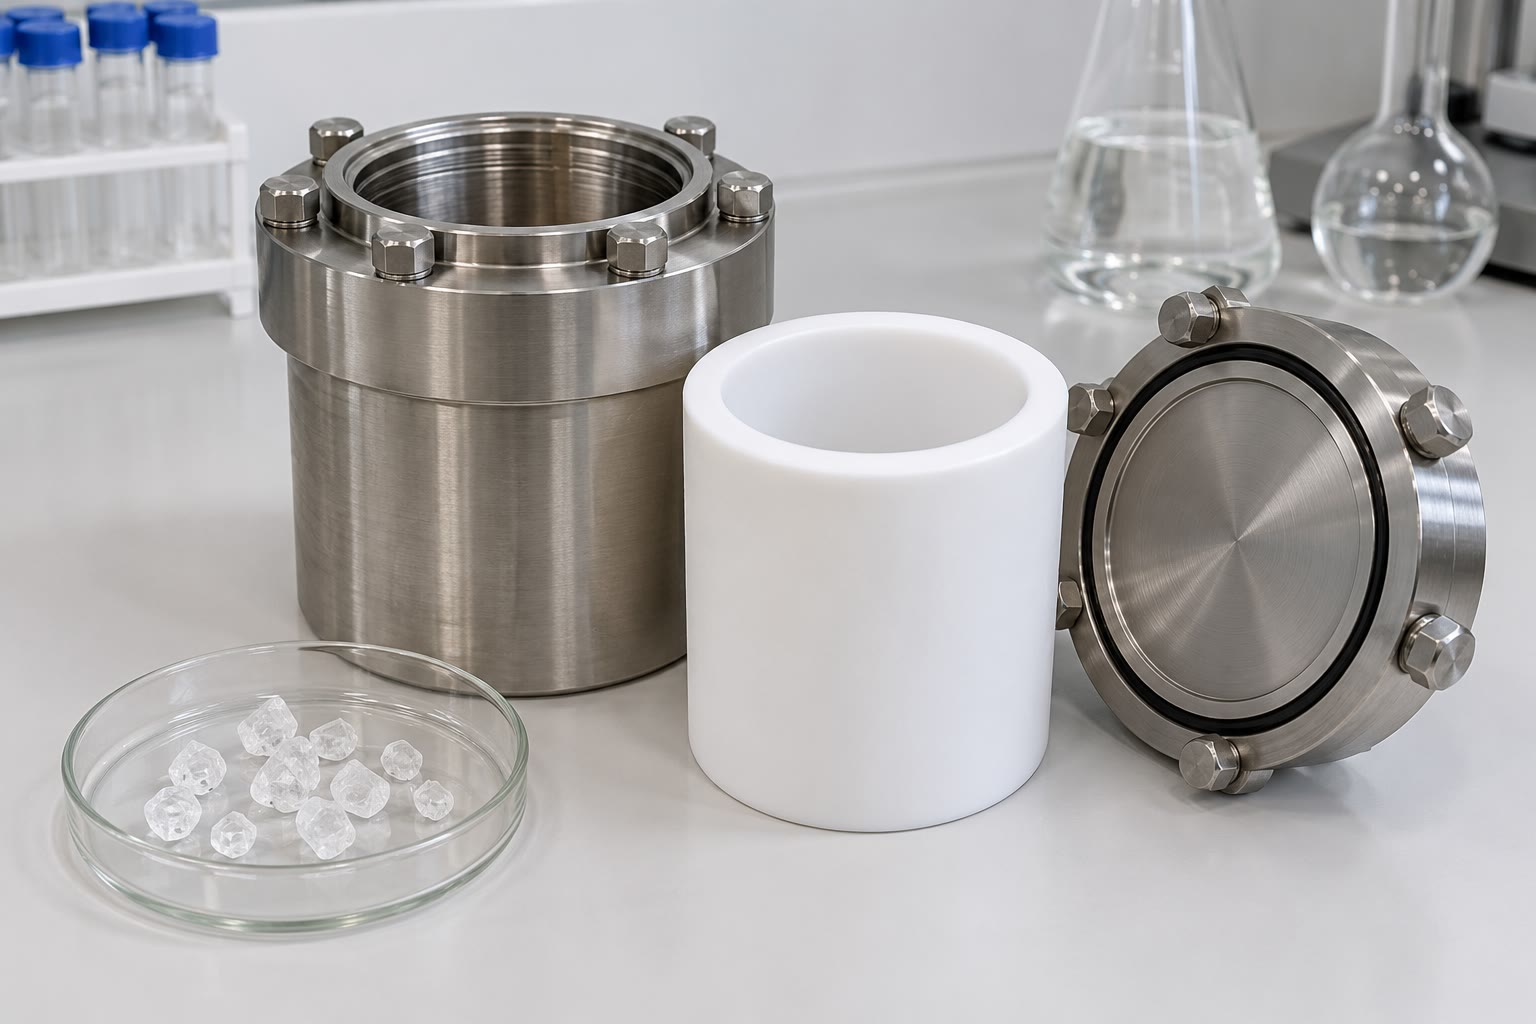
\includegraphics[width=0.5\linewidth]{images/book4/ai/b3-23-autoclave.jpg}

{\small Un autoclave de laboratorio para \omterm{def:b3:inorganic-materials:hydrothermal}{síntesis hidrotermal}: un cuerpo de acero con una
tapa atornillada, un vaso interior de polímero blanco que contiene la mezcla de reacción, y cristales
crecidos en él.}
\end{omfigure}

\section{Cerámicas y vidrios}

\begin{definition}[Cerámica]\label{def:b3:inorganic-materials:ceramic}
Una \emph{cerámica}\index{ceramica@cerámica} es un sólido inorgánico no metálico obtenido
calentando un polvo: óxidos, nitruros y carburos, o productos de arcilla.
\end{definition}

\begin{definition}[Estructura perovskita]\label{def:b3:inorganic-materials:perovskite}
La \emph{estructura perovskita}\index{estructura perovskita} de un óxido $\mathrm{ABO_3}$
tiene los cationes B pequeños en los centros de octaedros $\mathrm{BO_6}$ que comparten vértices y
los cationes A grandes en las cavidades de coordinación doce situadas entre ellos; en la
celda cúbica ideal, B está en el centro, O en los centros de las caras y A en los vértices.
El \emph{factor de tolerancia}\index{factor de tolerancia} mide lo bien que encajan
los iones:
\[
  t = \frac{r_A + r_O}{\sqrt2\,(r_B + r_O)}.
\]
\end{definition}

\begin{omfigure}
\tdplotsetmaincoords{60}{100}
\begin{tikzpicture}[tdplot_main_coords, scale=1.5, font=\small,
  aA/.style={om atom, ball color=green!45!black, minimum size=7.4mm},
  aB/.style={om atom, ball color=black!35, minimum size=4.4mm},
  aOs/.style={om atom, ball color=red!80, minimum size=4.8mm}]
  \pic[transform shape] {omcubeo={2}};
  % atoms back to front for view 60/100 (depth 0.853x + 0.150y + 0.5z)
  \node[aA] at (0,0,0) {};
  \node[aA] at (0,2,0) {};
  \node[aOs] (o1) at (0,1,1) {};
  \node[aA] at (0,0,2) {};
  \node[aOs] (o2) at (1,1,0) {};
  \node[aA] at (0,2,2) {};
  \node[aOs] (o3) at (1,0,1) {};
  \node[aB] (b) at (1,1,1) {};
  \node[aOs] (o4) at (1,2,1) {};
  \node[aA] at (2,0,0) {};
  \node[aOs] (o5) at (1,1,2) {};
  \node[aA] at (2,2,0) {};
  \node[aOs] (o6) at (2,1,1) {};
  \node[aA] at (2,0,2) {};
  \node[aA] at (2,2,2) {};
  \begin{scope}[on background layer]
    \draw[omMeth!70, line width=0.6pt] (o1.center) -- (o2.center) -- (o6.center) -- (o5.center) -- cycle
      (o3.center) -- (o2.center) -- (o4.center) -- (o5.center) -- cycle
      (o1.center) -- (o3.center) -- (o6.center) -- (o4.center) -- cycle;
    \draw[bond] (b.center) -- (o1.center) (b.center) -- (o2.center) (b.center) -- (o3.center)
      (b.center) -- (o4.center) (b.center) -- (o5.center) (b.center) -- (o6.center);
  \end{scope}
  \node[anchor=west] at (2,3.35,2) {A};
  \node[anchor=west] at (2,3.35,1) {O};
  \node[anchor=west] at (2,3.35,0) {B};
  \node[aA, minimum size=4mm] at (2,3.2,2) {};
  \node[aOs, minimum size=3.2mm] at (2,3.2,1) {};
  \node[aB, minimum size=3mm] at (2,3.2,0) {};
\end{tikzpicture}

{\small La celda cúbica de la perovskita $\mathrm{ABO_3}$: un catión B (gris) en el centro de un
octaedro de seis iones óxido situados en los centros de las caras (aristas verdes), y los cationes A
en los vértices. Cada ion A de un vértice está compartido por ocho celdas y cada oxígeno por
dos: un A, un B y tres O por celda.}
\end{omfigure}

\begin{proposition}[Factor de tolerancia ideal]\label{prop:b3:inorganic-materials:tolerance}
En la perovskita cúbica ideal, con los iones en contacto a lo largo de las direcciones B--O y A--O,
$t = 1$.
\end{proposition}

\begin{proof}
Con arista $a$, B en el centro y O en el centro de una cara están separados $a/2$: $r_B + r_O = a/2$.
A en un vértice y O en el centro de una cara adyacente están separados media diagonal
de cara: $r_A + r_O = a\sqrt2/2$. Dividiendo, $(r_A + r_O)/(r_B + r_O) = \sqrt2$, luego $t = 1$.
\end{proof}

Cuando $t$ es algo inferior a 1, el ion A es demasiado pequeño para su cavidad y los
octaedros se inclinan para cerrarse a su alrededor, lo que rebaja la simetría; cuando $t$ es superior a 1,
el ion B es demasiado pequeño para su octaedro y puede desplazarse del centro.

\begin{definition}[Ferroeléctrico]\label{def:b3:inorganic-materials:ferroelectric}
Un \emph{ferroeléctrico}\index{ferroelectrico@ferroeléctrico} es un cristal con una polarización
eléctrica espontánea que un campo eléctrico aplicado puede invertir.
\end{definition}

% ledger: rion:Ba2+XII, rion:Ti4+VI, rion:O2-VI
El titanato de bario es el caso clásico: con $r(\ce{Ba^2+}) = \qty{161}{pm}$ (coordinación doce),
$r(\ce{Ti^4+}) = \qty{60.5}{pm}$ y $r(\ce{O^2-}) = \qty{140}{pm}$, $t = 1.06$. Por debajo de una temperatura de transición, los
iones titanio se desplazan del centro, todos en la misma dirección dentro de un dominio,
y el cristal se polariza; la enorme permitividad cerca de la transición hace del
titanato de bario el dieléctrico de la mayoría de los condensadores cerámicos.

\begin{definition}[Vidrios de óxido]\label{def:b3:inorganic-materials:glass}
Un \emph{vidrio de óxido}\index{vidrio de oxido@vidrio de óxido} es un sólido de óxido amorfo, obtenido
enfriando un fundido sin cristalización. Sus \emph{formadores de
red}\index{formador de red} ($\ce{SiO2}$, $\ce{B2O3}$, $\ce{P2O5}$) construyen una red continua de
poliedros que comparten vértices; sus \emph{modificadores de red}\index{modificador de red}
($\ce{Na2O}$, $\ce{CaO}$) rompen puentes de esa red, y cada ion óxido añadido convierte un
oxígeno puente en dos no puente, con los cationes alojados en los
huecos.
\end{definition}

\begin{omfigure}
\begin{tikzpicture}
\begin{axis}[name=c, width=0.5\linewidth, axis equal image, hide axis, xmin=-1.2, xmax=12.6, ymin=-1.2, ymax=8.7]
\addplot[quiver={u=\thisrow{u}, v=\thisrow{v}}, -, black!60, line width=0.6pt] table {figdata/out/bachelor-3-glass-network-crystal-bonds.dat};
\addplot[only marks, mark=*, mark size=2.2pt, omDef] table {figdata/out/bachelor-3-glass-network-crystal-T.dat};
\addplot[only marks, mark=*, mark size=1.3pt, omThm, mark options={fill=white}] table {figdata/out/bachelor-3-glass-network-crystal-O.dat};
\end{axis}
\begin{axis}[at={(c.east)}, anchor=west, xshift=0.2cm, width=0.5\linewidth, axis equal image, hide axis, xmin=-1.2, xmax=12.6, ymin=-1.2, ymax=8.7]
\addplot[quiver={u=\thisrow{u}, v=\thisrow{v}}, -, black!60, line width=0.6pt] table {figdata/out/bachelor-3-glass-network-glass-bonds.dat};
\addplot[only marks, mark=*, mark size=2.2pt, omDef] table {figdata/out/bachelor-3-glass-network-glass-T.dat};
\addplot[only marks, mark=*, mark size=1.3pt, omThm, mark options={fill=white}] table {figdata/out/bachelor-3-glass-network-glass-O.dat};
\addplot[only marks, mark=*, mark size=1.5pt, omThm] table {figdata/out/bachelor-3-glass-network-glass-NBO.dat};
\addplot[only marks, mark=*, mark size=2.6pt, omProp] table {figdata/out/bachelor-3-glass-network-glass-Na.dat};
\end{axis}
\end{tikzpicture}

{\small Imagen bidimensional de un cristal y de un vidrio de la misma
composición (en azul: formadores tricoordinados; círculos rojos vacíos: oxígenos
puente). A la izquierda, el cristal repite un solo anillo. A la derecha, el vidrio: cada formador
sigue teniendo tres oxígenos a distancias casi iguales, pero los anillos tienen cinco,
seis o siete miembros y nada se repite; en dos lugares, un modificador ha roto un
puente y ha dejado dos oxígenos no puente (rojo lleno) y un catión (naranja) en
el hueco. Red modelo, relajada con resortes.}
\end{omfigure}

William Zachariasen sostuvo en 1932 que un óxido forma fácilmente un vidrio cuando su
catión está rodeado por pocos oxígenos (tres o cuatro), cada oxígeno une como máximo
dos cationes y los poliedros comparten vértices, no aristas ni caras: entonces una
red aleatoria apenas cuesta más energía que el cristal. El vidrio de ventana es
sílice con óxidos de sodio y de calcio como modificadores, que rebajan la temperatura de
fusión. El vidrio templado de las pantallas de los teléfonos se sumerge en nitrato de potasio
fundido: los iones $\ce{K+}$, más grandes, sustituyen a los iones $\ce{Na+}$ de la superficie y, al estar apretados,
la ponen en compresión, de modo que las grietas no se abren.

\section{Sólidos porosos: zeolitas y redes}

\begin{definition}[Zeolitas]\label{def:b3:inorganic-materials:zeolite}
Una \emph{zeolita}\index{zeolita} es un aluminosilicato cristalino cuyo
armazón de tetraedros $\ce{SiO4}$ y $\ce{AlO4}$ que comparten vértices encierra cavidades y
canales de tamaño molecular, con cationes intercambiables y agua en su interior. Un
\emph{tamiz molecular}\index{tamiz molecular} es un sólido poroso que admite
las moléculas según su tamaño; la \emph{selectividad de forma}\index{selectividad de forma}
es el control de una reacción por el tamaño y la forma de los poros en los
que tiene lugar.
\end{definition}

Cada tetraedro $\ce{AlO4}$ lleva una carga negativa más que un $\ce{SiO4}$
(aluminio(III) en lugar de silicio(IV)); los cationes de las cavidades, $\ce{Na+}$ o $\ce{Ca^2+}$,
la compensan y pueden intercambiarse.

\begin{proposition}[Regla de Löwenstein]\label{prop:b3:inorganic-materials:lowenstein}
En el armazón de una \omterm{def:b3:inorganic-materials:zeolite}{zeolita}, dos tetraedros $\ce{AlO4}$ nunca comparten un oxígeno: los enlaces Al--O--Al
están ausentes (una observación válida en todos los armazones de aluminosilicato conocidos). En
consecuencia, la razón Si/Al de una \omterm{def:b3:inorganic-materials:zeolite}{zeolita} es al menos 1.
\end{proposition}

\begin{proof}[Demostración de la consecuencia]
Cada aluminio tiene cuatro oxígenos, cada uno compartido con un silicio según la regla:
$4N_{\mathrm{Al}}$ enlaces Al--O--Si. Cada silicio tiene solo cuatro oxígenos, de modo que participa en
cuatro de esos enlaces como máximo: $4N_{\mathrm{Al}} \le 4N_{\mathrm{Si}}$, es decir, $N_{\mathrm{Si}}/N_{\mathrm{Al}} \ge 1$. La igualdad obliga a que cada
silicio tenga cuatro vecinos aluminio: el Si y el Al alternan.
\end{proof}

\begin{omfigure}
\tdplotsetmaincoords{55}{135}
\begin{tikzpicture}[tdplot_main_coords, scale=0.85, font=\small, baseline=(current bounding box.center),
  tSi/.style={circle, inner sep=0pt, minimum size=2.6mm, draw=black!70, fill=omDef!80},
  tAl/.style={circle, inner sep=0pt, minimum size=2.6mm, draw=black!70, fill=omProp!80}]
  % edges of a truncated octahedron (vertices: permutations of (0, +-1, +-2));
  % hidden edges (both faces facing away for this view) dashed
  \foreach \a/\b/\c/\d/\e/\f in {-2/-1/0/-2/0/-1, -2/-1/0/-2/0/1, -2/-1/0/-1/-2/0, -2/0/-1/-2/1/0, -2/0/-1/-1/0/-2, -1/-2/0/0/-2/-1, -1/-2/0/0/-2/1, -1/0/-2/0/-1/-2, -1/0/-2/0/1/-2, 0/-2/-1/0/-1/-2, 0/-2/-1/1/-2/0, 0/-1/-2/1/0/-2}
    \draw[black!40, dashed] (\a,\b,\c) -- (\d,\e,\f);
  \foreach \a/\b/\c/\d/\e/\f in {-2/0/1/-2/1/0, -2/0/1/-1/0/2, -2/1/0/-1/2/0, -1/0/2/0/-1/2, -1/0/2/0/1/2, -1/2/0/0/2/-1, -1/2/0/0/2/1, 0/-2/1/0/-1/2, 0/-2/1/1/-2/0, 0/-1/2/1/0/2, 0/1/-2/0/2/-1, 0/1/-2/1/0/-2, 0/1/2/0/2/1, 0/1/2/1/0/2, 0/2/-1/1/2/0, 0/2/1/1/2/0, 1/-2/0/2/-1/0, 1/0/-2/2/0/-1, 1/0/2/2/0/1, 1/2/0/2/1/0, 2/-1/0/2/0/-1, 2/-1/0/2/0/1, 2/0/-1/2/1/0, 2/0/1/2/1/0}
    \draw[black!75, line width=0.7pt] (\a,\b,\c) -- (\d,\e,\f);
  % T atoms back to front; hidden ones paler
  \foreach \x/\y/\z/\k/\v in {-2/-1/0/Si/0, -1/-2/0/Al/0, -2/0/-1/Al/0, 0/-2/-1/Si/0, -1/0/-2/Si/0, 0/-1/-2/Al/0, -2/0/1/Al/1, 0/-2/1/Si/1, -2/1/0/Si/1, 1/-2/0/Al/1, 0/1/-2/Al/1, 1/0/-2/Si/1, -1/0/2/Si/1, 0/-1/2/Al/1, -1/2/0/Al/1, 2/-1/0/Si/1, 0/2/-1/Si/1, 2/0/-1/Al/1, 0/1/2/Al/1, 1/0/2/Si/1, 0/2/1/Si/1, 2/0/1/Al/1, 1/2/0/Al/1, 2/1/0/Si/1}
    \node[t\k, opacity=0.35+0.65*\v] at (\x,\y,\z) {};
\end{tikzpicture}
\hspace{1.2cm}
\begin{tikzpicture}[font=\small, scale=0.8, baseline=(current bounding box.center)]
  \foreach \i in {0,1,2} \foreach \j in {0,1,2} {
    \fill[omDef!70] ($(2.2*\i,2.2*\j)+(-0.28,-0.28)$) rectangle +(0.56,0.56);
  }
  \foreach \i in {0,1} \foreach \j in {0,1,2} {
    \draw[black!70, line width=0.8pt] (2.2*\i+0.28,2.2*\j) -- (2.2*\i+0.75,2.2*\j);
    \draw[black!70, line width=0.8pt] (2.2*\i+1.45,2.2*\j) -- (2.2*\i+1.92,2.2*\j);
    \node[draw=black!70, regular polygon, regular polygon sides=6, minimum size=5.6mm, inner sep=0pt] at (2.2*\i+1.1,2.2*\j) {};
  }
  \foreach \i in {0,1,2} \foreach \j in {0,1} {
    \draw[black!70, line width=0.8pt] (2.2*\i,2.2*\j+0.28) -- (2.2*\i,2.2*\j+0.75);
    \draw[black!70, line width=0.8pt] (2.2*\i,2.2*\j+1.45) -- (2.2*\i,2.2*\j+1.92);
    \node[draw=black!70, regular polygon, regular polygon sides=6, minimum size=5.6mm, inner sep=0pt] at (2.2*\i,2.2*\j+1.1) {};
  }
  \node[font=\scriptsize, align=center] at (1.1,-0.85) {nodo $\ce{Zn4O}$ $+$ conector tereftalato};
\end{tikzpicture}

{\small Izquierda: una caja de sodalita, la unidad de construcción de la \omterm{def:b3:inorganic-materials:zeolite}{zeolita} A, con un
átomo tetraédrico en cada vértice (los oxígenos, en el centro de cada arista, no se
dibujan); el silicio (azul) y el aluminio (naranja) alternan, como exige la regla de Löwenstein
cuando Si/Al = 1. Derecha: una capa de una \omterm{def:b3:inorganic-materials:mof}{red metal--orgánica},
esquemática: agregados $\ce{Zn4O}$ (cuadrados) unidos por conectores benceno-1,4-dicarboxilato
(anillos) en una malla cúbica de poros grandes.}
\end{omfigure}

\begin{method}[Fórmula y capacidad de intercambio de una zeolita]\label{met:b3:inorganic-materials:zeolite-formula}
\begin{enumerate}
  \item Escribir el armazón como $\mathrm{[(AlO_2)_x(SiO_2)_y]^{x-}}$: Si/Al $= y/x$.
  \item La carga del armazón, $-x$, la compensan cationes: $x$ monovalentes o $x/2$
        divalentes.
  \item La capacidad de intercambio es la cantidad de carga intercambiable por gramo:
        $x/M$ moles de cationes monovalentes, $x/2M$ de divalentes, donde $M$ es la
        masa molar de la fórmula tal como se pesa (anhidra o hidratada).
\end{enumerate}
\end{method}

\begin{proposition}[Capacidad de intercambio]\label{prop:b3:inorganic-materials:exchange-capacity}
La capacidad de una \omterm{def:b3:inorganic-materials:zeolite}{zeolita} para un catión de carga $z$ es de $x/(zM)$ moles por gramo,
donde $x$ es el número de átomos de aluminio de una fórmula de masa molar $M$.
\end{proposition}

\begin{proof}
Cada aluminio aporta una carga negativa al armazón; la neutralidad
eléctrica exige $x$ unidades de carga positiva, todas ellas intercambiables, es decir,
$x/z$ cationes de carga $z$ por unidad fórmula, o sea, por masa $M$.
\end{proof}

% ledger: iza:LTA.window, iza:MFI.channels
La \omterm{def:b3:inorganic-materials:zeolite}{zeolita} A tiene ventanas de ocho tetraedros, de \qty{0.41}{nm} de anchura: el agua y los iones
pequeños pasan, y las moléculas ramificadas no. La ZSM-5 tiene dos sistemas de canales de diez
tetraedros, de unos 0.51 a \qty{0.56}{nm}: en la conversión del metanol o en la
alquilación del tolueno, el esbelto \textit{para}-xileno difunde hacia fuera mucho más deprisa que
sus isómeros \textit{orto} y \textit{meta}, que permanecen y se isomerizan. Eso es la
\omterm{def:b3:inorganic-materials:zeolite}{selectividad de forma}.

\begin{definition}[Redes metal--orgánicas]\label{def:b3:inorganic-materials:mof}
Una \emph{red metal--orgánica}\index{red metal--organica@red metal--orgánica} (MOF) es un
sólido cristalino formado por iones o agregados metálicos unidos por conectores
orgánicos politópicos en una red porosa. Una \emph{unidad de construcción
secundaria}\index{unidad de construccion secundaria@unidad de construcción secundaria} es el agregado metálico con sus
grupos coordinantes, tratado como un nodo de la red; la \emph{síntesis
reticular}\index{sintesis reticular@síntesis reticular} es el diseño de una red eligiendo
nodos y conectores de geometría dada de modo que se ensamblen en una red elegida.
\end{definition}

% ledger: cod:MOF5.formula, cod:MOF5.a
En el MOF-5, los agregados $\ce{Zn4O}$ con seis grupos carboxilato son nodos octaédricos,
y los conectores benceno-1,4-dicarboxilato los unen a lo largo de las aristas de una red
cúbica, $a = \qty{25.82}{\angstrom}$ para una celda de ocho nodos. Sustituir el conector por uno
más largo conserva la red y agranda los poros: esa es la idea reticular. Estas
redes tienen superficies de miles de metros cuadrados por gramo y se
estudian para almacenar hidrógeno y metano y para capturar dióxido de carbono.

\begin{definition}[Tamaños de poro]\label{def:b3:inorganic-materials:pores}
% ledger: pore:micro, pore:macro
Por convenio, los \emph{microporos}\index{microporo} miden menos de \qty{2}{nm},
los \emph{mesoporos}\index{mesoporo} entre 2 y \qty{50}{nm}, y
los \emph{macroporos}\index{macroporo} más de \qty{50}{nm}.
\end{definition}

Las \omterm{def:b3:inorganic-materials:zeolite}{zeolitas} y la mayoría de los MOF son microporosos; los \omterm{def:b3:colloids:colloid}{geles} de sílice y los \omterm{def:b3:inorganic-materials:sol-gel}{aerogeles}, mesoporosos.

\section{Nanopartículas}

\begin{definition}[Nanomateriales]\label{def:b3:inorganic-materials:nano}
Un \emph{nanomaterial}\index{nanomaterial} tiene al menos una dimensión comprendida entre
1 y \qty{100}{nm} aproximadamente; una \emph{nanopartícula}\index{nanoparticula@nanopartícula} tiene las
tres.
\end{definition}

\begin{proposition}[Agregados mágicos]\label{prop:b3:inorganic-materials:magic}
Un agregado cuboctaédrico formado por un átomo central y $n$ capas completas tiene
\[
  N(n) = \frac{10n^3 + 15n^2 + 11n + 3}{3}
\]
átomos, de los cuales $10n^2 + 2$ están en la superficie: 13, 55, 147, 309, \dots
\end{proposition}

\begin{proof}
La $k$-ésima capa de un cuboctaedro tiene 12 vértices, 24 aristas con $k - 1$ átomos
en el interior de cada una, 8 caras triangulares con $(k - 1)(k - 2)/2$ átomos interiores cada una y 6
caras cuadradas con $(k - 1)^2$: en total, $12 + 24(k - 1) + 4(k - 1)(k - 2) + 6(k - 1)^2 = 10k^2 + 2$. Entonces
$N(n) = 1 + \sum_{k=1}^{n}(10k^2 + 2) = 1 + \frac{10n(n + 1)(2n + 1)}{6} + 2n$, que al desarrollarse da la fórmula; la
capa exterior, de $10n^2 + 2$ átomos, es la superficie.
\end{proof}

\begin{omfigure}
\begin{tikzpicture}
\begin{axis}[name=a, width=0.47\linewidth, height=5.4cm, xmin=0, xmax=18, ymin=0, ymax=1,
  axis lines=left, xlabel={diámetro / \unit{nm}}, ylabel={fracción de átomos en la superficie},
  tick label style={font=\scriptsize}, label style={font=\small}]
\addplot[omDef, thick, mark=*, mark size=1pt] table[x=diam_nm, y=fsurf] {figdata/out/bachelor-3-nanoparticle-size.dat};
\end{axis}
\begin{axis}[at={(a.east)}, anchor=west, xshift=1.5cm, width=0.47\linewidth, height=5.4cm,
  xmin=0.8, xmax=6, ymin=0, ymax=3, axis lines=left,
  xlabel={radio $R$ / \unit{nm}}, ylabel={energía de confinamiento / \unit{eV}},
  tick label style={font=\scriptsize}, label style={font=\small}]
\addplot[omThm, thick] table[x=R_nm, y=dE_eV] {figdata/out/bachelor-3-nanoparticle-size-b.dat};
\end{axis}
\end{tikzpicture}

{\small Izquierda: fracción de átomos en la superficie de agregados cuboctaédricos de oro
en función de su diámetro: más de la mitad para agregados de menos de unos
\qty{3}{nm}, y todavía una quinta parte a \qty{8}{nm}. Derecha: energía de confinamiento de un
par electrón--hueco en un \omterm{def:b3:inorganic-materials:quantum-dot}{punto cuántico} esférico (\omterm{def:b3:quantum-model-systems:oscillator}{masa reducida} del modelo, $0.10\,m_e$),
que se suma a la \omterm{def:b3:solid-state:band}{banda prohibida} y decrece como $1/R^2$.}
\end{omfigure}

Con una gran fracción de sus átomos en la superficie, donde tienen menos
vecinos, una \omterm{def:b3:inorganic-materials:nano}{nanopartícula} funde a una temperatura más baja que el metal masivo,
es más reactiva y puede ser un catalizador mucho mejor: el oro masivo es inerte, y las partículas
de oro de unos pocos nanómetros oxidan el monóxido de carbono a temperatura ambiente.

\begin{definition}[Puntos cuánticos]\label{def:b3:inorganic-materials:quantum-dot}
Un \emph{punto cuántico}\index{punto cuantico@punto cuántico} es un nanocristal \omterm{def:b3:solid-state:classes}{semiconductor} lo bastante
pequeño para que el confinamiento de sus electrones y de sus \omterm{def:b3:solid-state:carriers}{huecos} eleve su \omterm{def:b3:solid-state:band}{banda prohibida}
por encima de la del sólido masivo.
\end{definition}

\begin{theorem}[Confinamiento en una esfera]\label{thm:b3:inorganic-materials:quantum-dot}
Una partícula de masa $m$ confinada en una esfera de radio $R$ por paredes infinitas tiene
la energía del estado fundamental $E = \hbar^2\pi^2/(2mR^2) = h^2/(8mR^2)$, con la función de onda $\psi \propto \sin(\pi r/R)/r$.
\end{theorem}

\begin{proof}
Para un estado de simetría esférica, $\psi(r) = u(r)/r$, el laplaciano da
$\nabla^2\psi = u''/r$, de modo que la \omterm{thm:b3:quantum-model-systems:schrodinger}{ecuación de Schrödinger} en el interior se convierte en $-\frac{\hbar^2}{2m}u'' = Eu$, la de una partícula en una
recta. La solución con $\psi$ finita en el centro tiene $u(0) = 0$: $u = \sin(kr)$, con $E = \hbar^2k^2/2m$.
La pared exige $u(R) = 0$, luego $kR = \pi$ para el estado fundamental, y $E = \hbar^2\pi^2/(2mR^2)$.
\end{proof}

En un punto, el electrón y el \omterm{def:b3:solid-state:carriers}{hueco} están ambos confinados; la energía de la
excitación más baja es $E_g + h^2/(8\mu R^2)$ en primera aproximación, donde $\mu$ es su \omterm{def:b3:quantum-model-systems:oscillator}{masa
reducida} (su atracción de Coulomb la rebaja un poco). Reducir el radio a la mitad
multiplica por cuatro la energía de confinamiento: los puntos de seleniuro de cadmio de unos pocos
nanómetros brillan en rojo, verde o azul solo según su tamaño, y se usan como
emisores en las pantallas.

\begin{definition}[Resonancia de plasmón superficial]\label{def:b3:inorganic-materials:plasmon}
Una \emph{resonancia de plasmón superficial}\index{resonancia de plasmon superficial@resonancia de plasmón superficial} es una
oscilación colectiva de los electrones de conducción de una \omterm{def:b3:inorganic-materials:nano}{nanopartícula} metálica
excitada por la luz; da una banda de absorción intensa cuya longitud de onda depende
del metal, del tamaño y la forma de la partícula y de su entorno.
\end{definition}

Las \omterm{def:b3:inorganic-materials:nano}{nanopartículas} de oro de unas decenas de nanómetros absorben la luz verde y se ven
de color rojo rubí en un vidrio o en un \omterm{def:b3:colloids:colloid}{coloide}; cuando se agregan, la banda se desplaza hacia longitudes
de onda mayores y el color vira al azul: la base de muchos tests rápidos, en los que
un \omterm{def:b3:colloids:colloid}{coloide} de oro recubierto de anticuerpos se concentra en una línea coloreada.

\section{Nanomateriales de carbono}

\begin{definition}[Nanomateriales de carbono]\label{def:b3:inorganic-materials:carbon}
Un \emph{fullereno}\index{fullereno} es una molécula en forma de jaula cerrada de átomos de carbono,
cada uno unido a otros tres, con anillos de cinco y de seis miembros, como el
$\ce{C60}$ icosaédrico. Un \emph{nanotubo de carbono}\index{nanotubo de carbono} es una lámina de
grafito enrollada en un cilindro sin costura de alrededor de un nanómetro de diámetro.
El \emph{grafeno}\index{grafeno} es una sola capa de grafito, de un átomo de espesor.
\end{definition}

\begin{proposition}[Doce pentágonos]\label{prop:b3:inorganic-materials:euler}
Todo \omterm{def:b3:inorganic-materials:carbon}{fullereno} tiene exactamente doce pentágonos, sea cual sea su número de
hexágonos.
\end{proposition}

\begin{proof}
Una jaula cerrada es un poliedro: se cumple la fórmula de Euler, $V - E + F = 2$. Cada átomo tiene
tres enlaces y cada enlace, dos átomos: $2E = 3V$. Con $p$ pentágonos y $h$ hexágonos,
contar las aristas por caras da $2E = 5p + 6h$, y $F = p + h$. Entonces $V = 2E/3$, y la fórmula de
Euler se escribe $-E/3 + p + h = 2$, es decir, $-(5p + 6h)/6 + p + h = 2$, luego $p/6 = 2$: $p = 12$.
\end{proof}

\begin{omfigure}
\begin{tikzpicture}[scale=0.62, font=\small]
  \def\hexd{0.6}
  \begin{scope}
    \clip (-0.4,-0.5) rectangle (9.6,5.2);
    \foreach \i in {-3,...,10} \foreach \j in {-1,...,6} {
      \pgfmathsetmacro\cx{1.7320508*\hexd*(\i + 0.5*\j)}
      \pgfmathsetmacro\cy{1.5*\hexd*\j}
      \draw[black!45] ({\cx+\hexd*cos(30)},{\cy+\hexd*sin(30)})
        \foreach \k in {90,150,...,390} { -- ({\cx+\hexd*cos(\k)},{\cy+\hexd*sin(\k)}) };
    }
  \end{scope}
  \draw[->, thick, omDef] (0,0) -- ({1.7320508*\hexd},0) node[below right, font=\scriptsize, fill=white, inner sep=1pt] {$\mathbf a_1$};
  \draw[->, thick, omDef] (0,0) -- ({1.7320508*\hexd*0.5},{1.5*\hexd}) node[left, font=\scriptsize, fill=white, inner sep=1pt] {$\mathbf a_2$};
  \draw[->, very thick, omThm] (0,0) -- ({1.7320508*\hexd*(4+0.5*2)},{1.5*\hexd*2}) node[above right, font=\scriptsize, fill=white, inner sep=1pt] {$\mathbf C_h = 4\mathbf a_1 + 2\mathbf a_2$};
  \draw[dashed, omMeth, thick] (0,0) -- ({1.7320508*\hexd*9},0) node[right, font=\scriptsize] {zigzag $(n, 0)$};
  \draw[dashed, omProp, thick] (0,0) -- ({1.7320508*\hexd*5*1.5},{1.5*\hexd*5}) node[below right, font=\scriptsize, fill=white, inner sep=1pt] {sillón $(n, n)$};
\end{tikzpicture}

{\small Una lámina de \omterm{def:b3:inorganic-materials:carbon}{grafeno} y el vector quiral de un nanotubo: enrollar la lámina
de modo que el extremo de $\mathbf C_h = n\mathbf a_1 + m\mathbf a_2$ coincida con su origen da el tubo $(n, m)$, aquí $(4, 2)$.
A lo largo de $\mathbf a_1$, el borde de un tubo $(n, 0)$ es un zigzag; a lo largo de $\mathbf a_1 + \mathbf a_2$, a 30°, el de un tubo $(n, n)$
es un sillón.}
\end{omfigure}

\begin{proposition}[Nanotubos metálicos y semiconductores]\label{prop:b3:inorganic-materials:nanotube}
Un \omterm{def:b3:inorganic-materials:carbon}{nanotubo de carbono} de pared simple $(n, m)$ es metálico cuando $n - m$ es múltiplo de 3, y
\omterm{def:b3:solid-state:classes}{semiconductor} en los demás casos. \admitted
\end{proposition}

Un tercio de todos los tubos posibles son, pues, metálicos, entre ellos todos los tubos
sillón; la \omterm{def:b3:solid-state:band}{banda prohibida} de los demás disminuye a medida que crece su diámetro. El propio \omterm{def:b3:inorganic-materials:carbon}{grafeno} no tiene
ninguna \omterm{def:b3:solid-state:band}{banda prohibida}: sus \omterm{def:b3:solid-state:band}{bandas de valencia} y de conducción se tocan en puntos aislados, y sus
electrones se mueven como si no tuvieran masa.

\begin{safety}{\ghs[0.62cm]{GHS02}\ghs[0.62cm]{GHS07}\ghs[0.62cm]{GHS08}}
% ledger: ghs4:TEOS
Ortosilicato de tetraetilo: líquido y vapores inflamables, nocivo en caso de inhalación,
irritante para los ojos y las vías respiratorias; se manipula en una vitrina. Nanopolvos: las
partículas más finas llegan hasta el fondo de los pulmones, y muchas aún no están clasificadas;
se pesan y se manipulan en un recinto cerrado o en suspensión, nunca como un
polvo suelto al aire libre.
\end{safety}

\begin{omfigure}
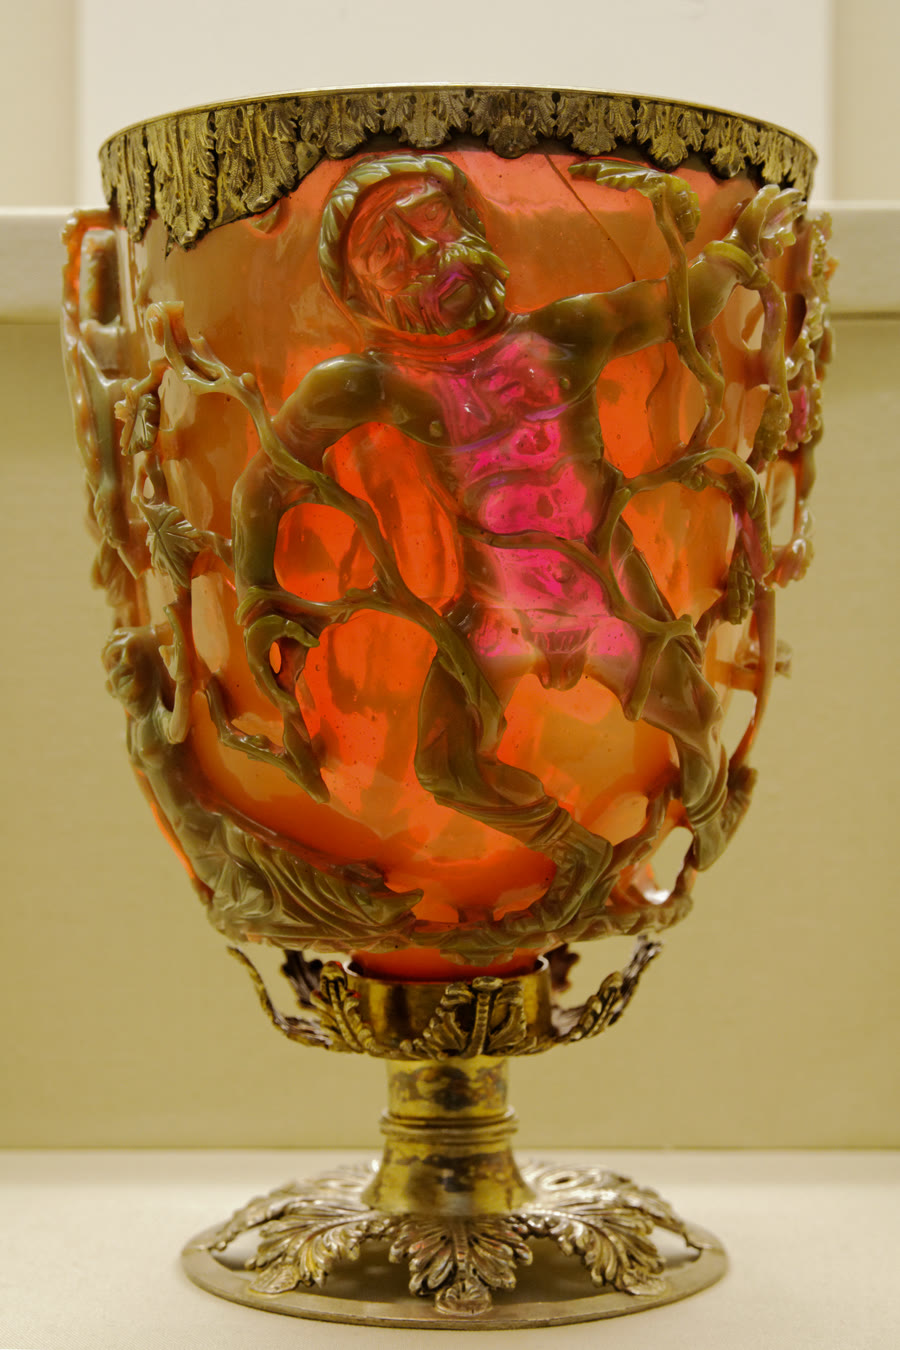
\includegraphics[width=0.32\linewidth]{images/book4/lycurgus-cup.jpg}

{\small La copa de Licurgo, un vidrio romano del siglo IV, iluminada desde dentro:
se ve verde con luz reflejada y roja con luz transmitida, un efecto de las
\omterm{def:b3:inorganic-materials:nano}{nanopartículas} de oro--plata del vidrio. Fotografía: Marie-Lan Nguyen, CC BY
2.5.}
\end{omfigure}

\begin{history}[Nanopartículas antes de la palabra, y un balón de carbono]
Los vidrieros coloreaban el vidrio de rojo con oro mucho antes de que nadie supiera por qué; la
copa de Licurgo muestra el efecto en su forma más llamativa. Michael Faraday preparó \omterm{def:b3:colloids:colloid}{coloides}
de oro en la década de 1850 y vio que su color se debía a partículas demasiado pequeñas
para verse. En 1985, Harold Kroto, Robert Curl y Richard Smalley, vaporizando
grafito con un láser, descubrieron que los agregados de sesenta átomos de carbono eran
excepcionalmente estables y propusieron la jaula cerrada de doce pentágonos y
veinte hexágonos; recibieron el Premio Nobel de Química de 1996.
\end{history}

\section{Ejercicios}

\begin{exercise}[$\star$]\label{exo:b3:inorganic-materials:1}
Una capa de producto entre dos sólidos tiene un espesor de \qty{2.0}{\micro\metre} al cabo de \qty{10}{h}. ¿Cuánto tarda en
alcanzar \qty{6.0}{\micro\metre}, si el crecimiento es parabólico?
\end{exercise}

\begin{exercise}[$\star$]\label{exo:b3:inorganic-materials:2}
Escríbanse la hidrólisis del ortosilicato de tetraetilo a ácido silícico, la
condensación de dos moléculas de ácido silícico y la reacción global que da
sílice.
\end{exercise}

\begin{exercise}[$\star$]\label{exo:b3:inorganic-materials:3}
Clasifíquense $\ce{SiO2}$, $\ce{B2O3}$, $\ce{Na2O}$ y $\ce{CaO}$ como formadores o \omterm{def:b3:inorganic-materials:glass}{modificadores de red}, y dígase qué
le hace el $\ce{Na2O}$ a la red de la sílice.
\end{exercise}

\begin{exercise}[$\star$]\label{exo:b3:inorganic-materials:4}
¿Cuántos pentágonos y hexágonos tiene el $\ce{C70}$? ¿Cuántos enlaces?
\end{exercise}

\begin{exercise}[$\star\star$]\label{exo:b3:inorganic-materials:5}
% ledger: rion:Sr2+XII, rion:Ca2+XII, rion:Ba2+XII, rion:Ti4+VI, rion:O2-VI
Calcúlense los \omterm{def:b3:inorganic-materials:perovskite}{factores de tolerancia} de $\ce{SrTiO3}$, $\ce{BaTiO3}$ y $\ce{CaTiO3}$ con los radios en coordinación doce
de $\ce{Sr^2+}$ (\qty{144}{pm}), $\ce{Ba^2+}$ (\qty{161}{pm}) y $\ce{Ca^2+}$ (\qty{134}{pm}), $r(\ce{Ti^4+}) = \qty{60.5}{pm}$ y $r(\ce{O^2-}) = \qty{140}{pm}$. ¿Qué
predicen?
\end{exercise}

\begin{exercise}[$\star\star$]\label{exo:b3:inorganic-materials:6}
Una \omterm{def:b3:inorganic-materials:zeolite}{zeolita} X tiene la fórmula anhidra $\mathrm{Na_{86}[(AlO_2)_{86}(SiO_2)_{106}]}$ (datos del ejercicio).
Dense la razón Si/Al y su capacidad de intercambio para el $\ce{Ca^2+}$ en milimoles por gramo.
\end{exercise}

\begin{exercise}[$\star\star$]\label{exo:b3:inorganic-materials:7}
% ledger: lat:Au
El oro es cúbico centrado en las caras, con $a = \qty{407.8}{pm}$. Estímense el número de capas de una
partícula cuboctaédrica de oro de unos \qty{5}{nm} de diámetro, su número de átomos y la
fracción que está en su superficie.
\end{exercise}

\begin{exercise}[$\star\star$]\label{exo:b3:inorganic-materials:8}
Un \omterm{def:b3:solid-state:classes}{semiconductor} tiene una \omterm{def:b3:solid-state:band}{banda prohibida} masiva de \qty{1.74}{eV}, y su electrón y su \omterm{def:b3:solid-state:carriers}{hueco}, una \omterm{def:b3:quantum-model-systems:oscillator}{masa
reducida} de $0.10\,m_e$ (datos del ejercicio). Estímese el color de la luz emitida por
puntos de radio 2.0 y \qty{3.0}{nm}, despreciando la atracción de Coulomb.
\end{exercise}

\begin{exercise}[$\star\star$]\label{exo:b3:inorganic-materials:9}
¿Son metálicos o \omterm{def:b3:solid-state:classes}{semiconductores} los nanotubos $(10, 10)$, $(10, 0)$, $(9, 0)$ y $(12, 8)$? ¿Cuáles
son de tipo sillón y cuáles de tipo zigzag?
\end{exercise}

\begin{exercise}[$\star\star\star$]\label{exo:b3:inorganic-materials:10}
% ledger: cod:MOF5.formula, cod:MOF5.a, cod:MOF5.Z
El MOF-5, $\mathrm{Zn_4O(C_8H_4O_4)_3}$, es cúbico, con $a = \qty{25.82}{\angstrom}$ y ocho unidades fórmula por celda.
Calcúlese su densidad. Si un gramo tiene una superficie de $\qty{3000}{m^2}$ (datos del
ejercicio), ¿a cuántos campos de fútbol de $\qty{105}{m} \times \qty{68}{m}$ equivale?
\end{exercise}

\begin{exercise}[$\star\star\star$]\label{exo:b3:inorganic-materials:11}
Con el recuento de capas de la \cref{prop:b3:inorganic-materials:magic}, demuéstrese que la
fracción superficial de un agregado cuboctaédrico tiende a $3/n$ para $n$ grande, y
compárese con la fracción exacta para $n = 8$.
\end{exercise}

\begin{exercise}[$\star\star\star$]\label{exo:b3:inorganic-materials:12}
Una jaula cerrada de carbono con tres enlaces por átomo contiene $p$ pentágonos, $h$ hexágonos
y $s$ heptágonos. Demuéstrese que $p - s = 12$.
\end{exercise}

\section{Problema: ablandar el agua con zeolita A}

\begin{problem}[{Problema de fin de semana --- ablandar el agua con zeolita A: la
fórmula y la regla de Löwenstein, la capacidad de intercambio teórica, la zeolita
necesaria para un lavado y la ventana que deja entrar el calcio y deja fuera los
detergentes}]
\label{pb:b3:inorganic-materials:1}
% ledger: iza:LTA.formula, iza:LTA.window, aw:Na, aw:Al, aw:Si, aw:O, aw:H, aw:Ca, aw:C, rion:Ca2+VI
La \omterm{def:b3:inorganic-materials:zeolite}{zeolita} A, usada en los detergentes en lugar de los fosfatos, tiene la fórmula
$\mathrm{Na_{12}[(AlO_2)_{12}(SiO_2)_{12}]\cdot 27H_2O}$ y ventanas de \qty{0.41}{nm} de anchura. Un agua del grifo contiene
\qty{2.0}{mmol/L} de $\ce{Ca^2+}$, y un lavado usa \qty{15}{L} de ella; en el tiempo de un lavado, la \omterm{def:b3:inorganic-materials:zeolite}{zeolita}
alcanza el 60\,\% de su capacidad (datos del problema).

\medskip\noindent\textbf{Parte I --- La fórmula.}
\begin{enumerate}
  \item Calcúlese la masa molar de la fórmula anhidra.
  \item Calcúlese la de la fórmula hidratada.
  \item Dese la razón Si/Al.
  \item Enúnciese la regla de Löwenstein y lo que implica aquí para la disposición del
        Si y del Al.
  \item ¿Cuál es la carga del armazón por fórmula?
  \item Calcúlese la fracción másica de agua de la \omterm{def:b3:inorganic-materials:zeolite}{zeolita} hidratada.
\end{enumerate}

\medskip\noindent\textbf{Parte II --- Capacidad de intercambio.}
\begin{enumerate}[resume]
  \item Escríbase el equilibrio de intercambio entre la \omterm{def:b3:inorganic-materials:zeolite}{zeolita} sódica y los iones
        calcio.
  \item ¿Cuántos $\ce{Ca^2+}$ puede captar una fórmula?
  \item Calcúlese la capacidad teórica de la \omterm{def:b3:inorganic-materials:zeolite}{zeolita} anhidra en mmol de $\ce{Ca^2+}$
        por gramo.
  \item Calcúlese para la \omterm{def:b3:inorganic-materials:zeolite}{zeolita} hidratada.
  \item Exprésese la capacidad anhidra en miligramos de $\ce{CaCO3}$ por gramo, la unidad
        habitual de la dureza del agua.
\end{enumerate}

\medskip\noindent\textbf{Parte III --- Un lavado.}
\begin{enumerate}[resume]
  \item Calcúlese la cantidad de $\ce{Ca^2+}$ en el agua de un lavado.
  \item Calcúlese la masa de \omterm{def:b3:inorganic-materials:zeolite}{zeolita} hidratada necesaria con la capacidad teórica.
  \item Calcúlese con el 60\,\% de la capacidad.
  \item Calcúlese la masa de sodio liberada al agua.
  \item ¿Por qué los fabricantes de detergentes sustituyeron los fosfatos?
  \item ¿Por qué la \omterm{def:b3:inorganic-materials:zeolite}{zeolita} A capta el $\ce{Mg^2+}$ más lentamente que el $\ce{Ca^2+}$?
\end{enumerate}

\medskip\noindent\textbf{Parte IV --- La ventana.}
\begin{enumerate}[resume]
  \item Compárese la ventana con el diámetro de un ion $\ce{Ca^2+}$ (radio en coordinación seis:
        \qty{100}{pm}).
  \item ¿Qué debe hacer un ion $\ce{Ca^2+}$ hidratado para pasar?
  \item ¿Por qué un anión \omterm{def:b3:colloids:surfactant}{tensioactivo} como el dodecilsulfato se queda fuera?
  \item ¿Qué hace la \omterm{def:b3:inorganic-materials:zeolite}{zeolita} A como agente desecante, y por qué se la llama
        \omterm{def:b3:inorganic-materials:zeolite}{tamiz molecular}?
  \item ¿Cómo cambiaría el tamaño de las moléculas admitidas la sustitución del $\ce{Na+}$ por $\ce{K+}$?
  \item En la ZSM-5, ¿por qué el \textit{para}-xileno sale de los poros más deprisa que el \textit{orto}-xileno?
  \item Enúnciese el resultado: la capacidad de intercambio teórica de la \omterm{def:b3:inorganic-materials:zeolite}{zeolita} A anhidra
        para el $\ce{Ca^2+}$.
\end{enumerate}
\end{problem}
